\section*{Problem 1} \label{sec:problem1}


% problem introduction
\begin{tcolorbox}[colback=red!5!white,boxrule=0pt,frame empty]
    Use wavelet decomposition (\verb|wavedec|) to decompose an audio signal (\verb|Q1.mat|, sample rate \verb|8192| Hz)
    three level decomposition using \verb|db1|.
\end{tcolorbox}

\vspace{0.5cm}

\begin{figure}[H]
    \centering
    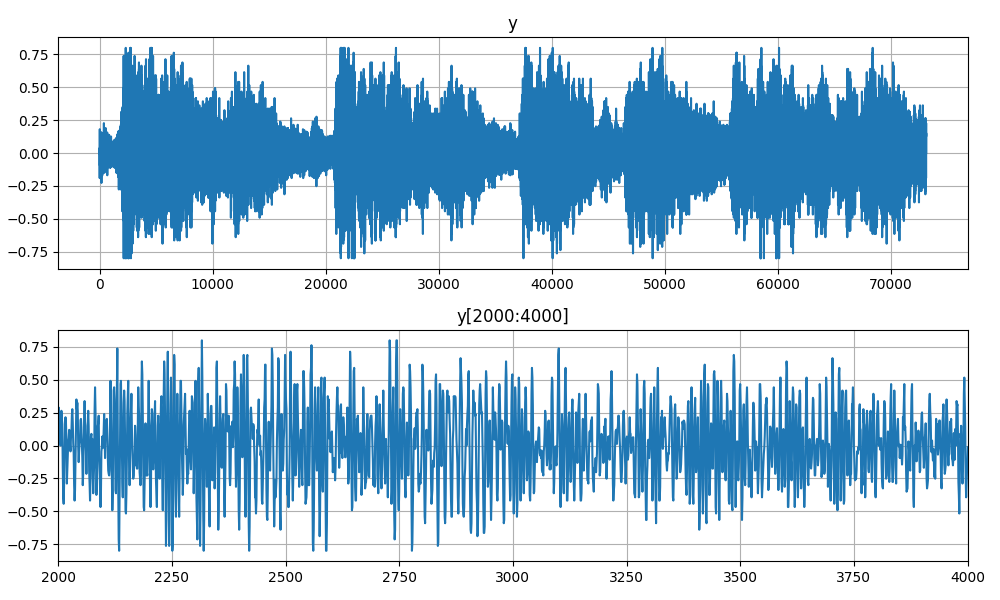
\includegraphics[width=\textwidth]{./img/Q1.png}
    \caption{The audio signal stored in $y$, sample rate 8192 Hz.}
    \label{fig:Q1}
\end{figure}

\vspace{0.5cm}


\begin{tcolorbox}[colback=red!5!white,colframe=red!75!black,title=Problem 1.a]
    Plot the approximated and detailed coefficients.
\end{tcolorbox}


\begin{figure}[H]
    \centering
    % thanks Jens
    \makebox[\textwidth][c]{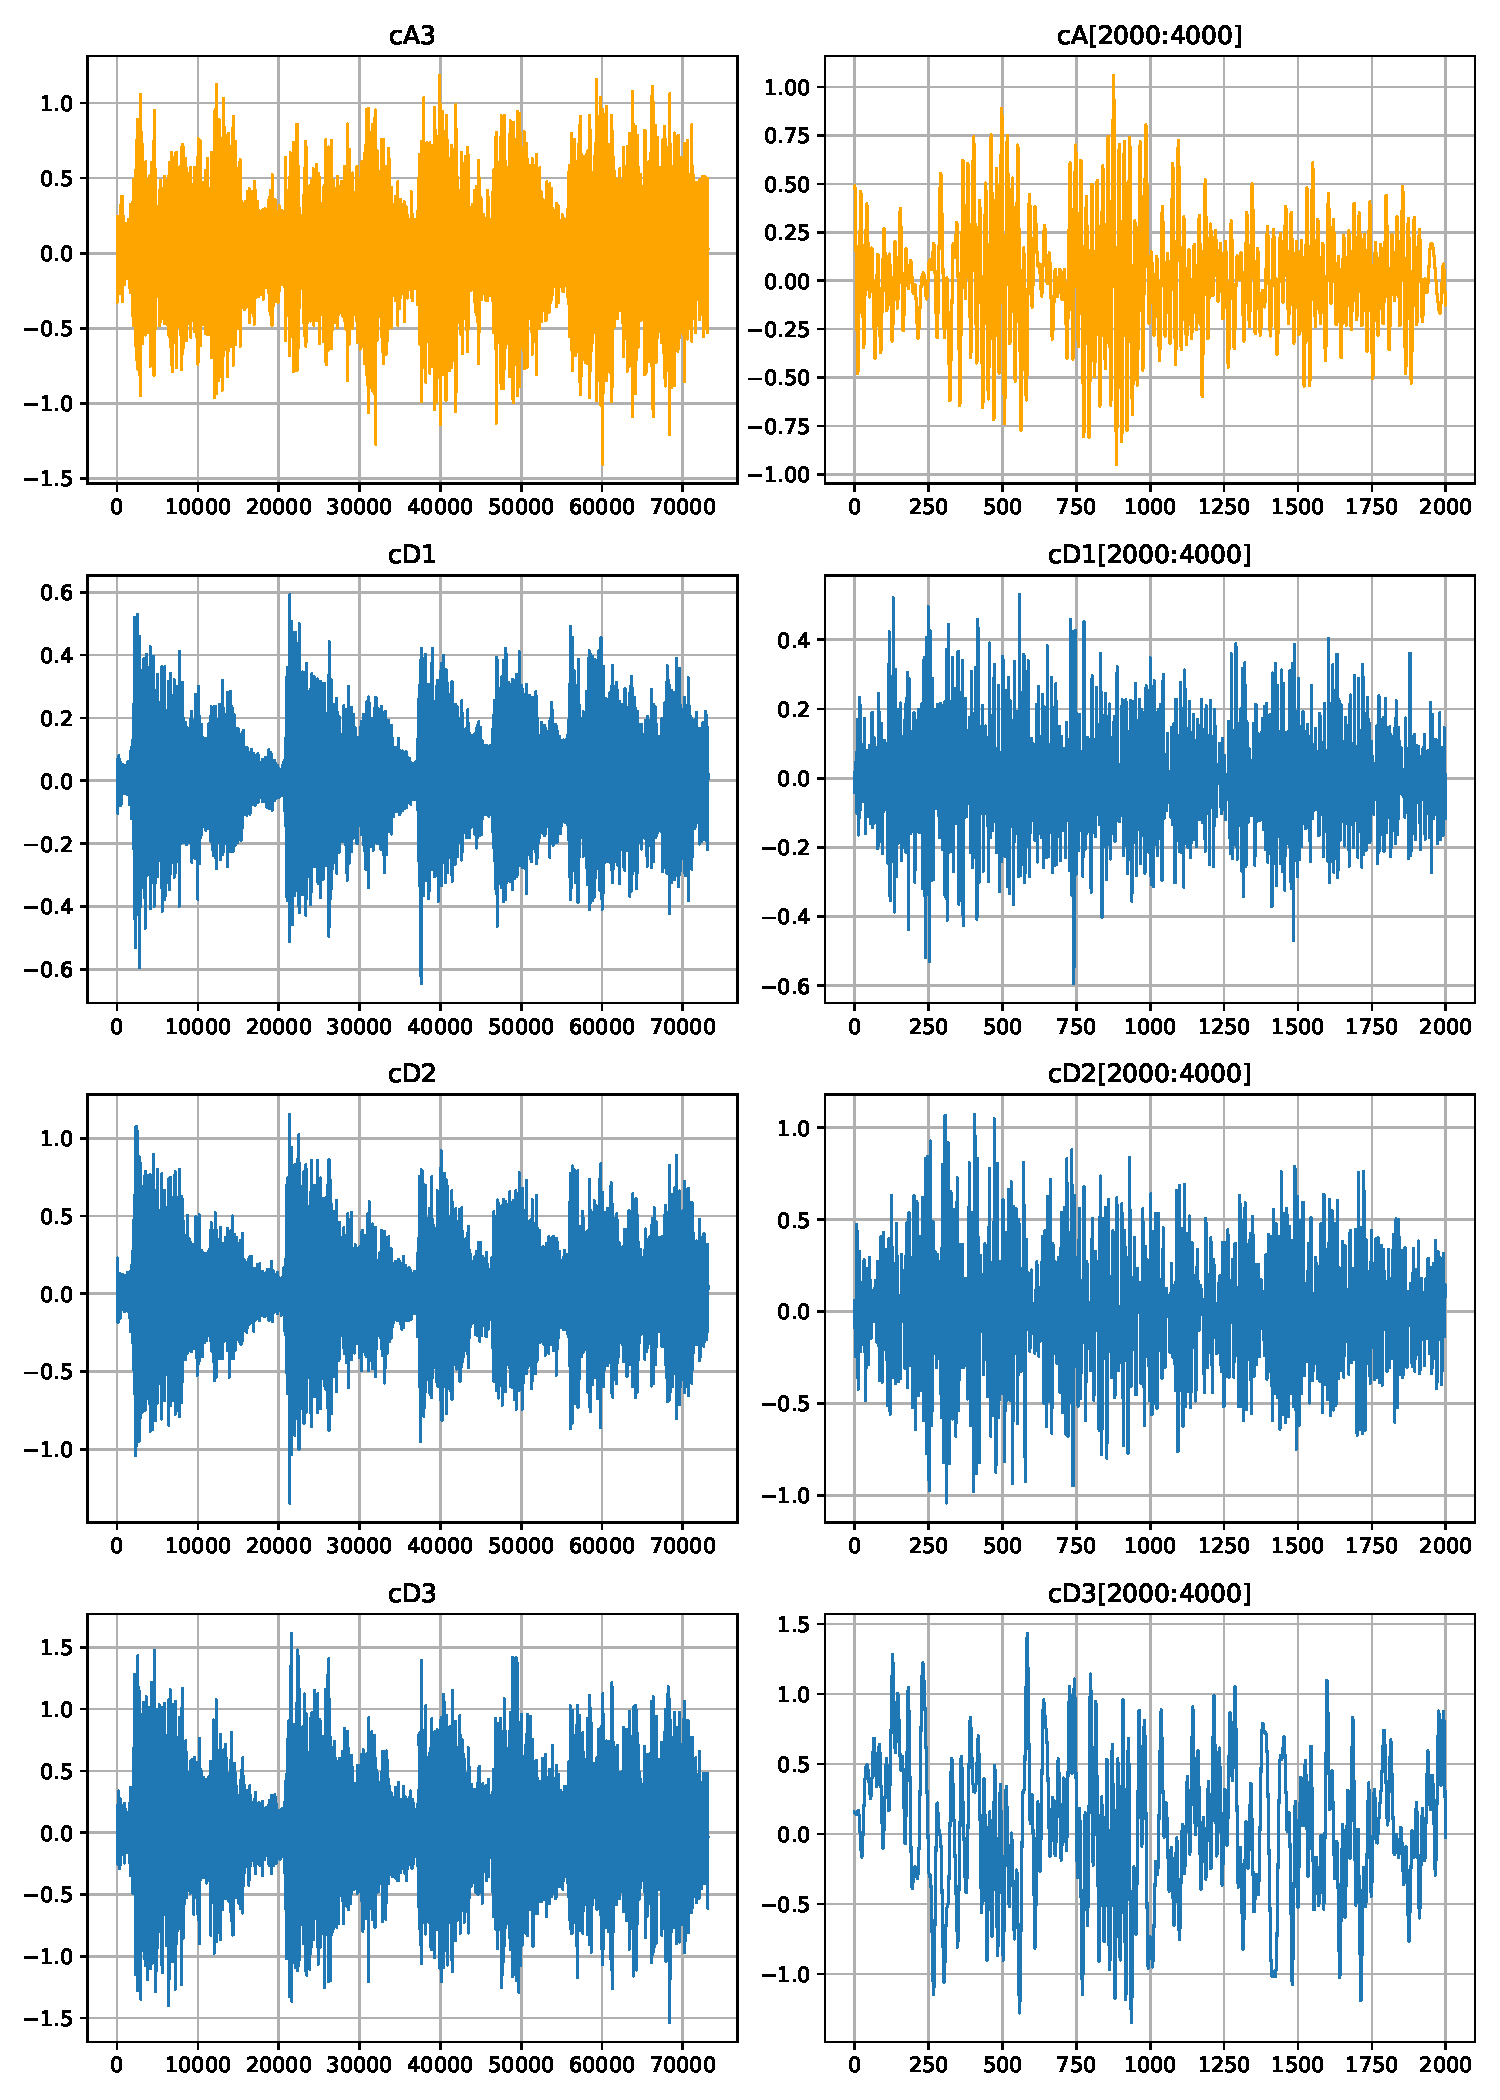
\includegraphics[width=1.1\textwidth]{./img/problem1-1-approximated-and-detailed-coeffs.pdf}}

    \caption{Approximated and detailed coefficients using DWT with \textit{db1} wavelet \textbf{6} levels deep. \todo{fix the y-axis limits.}}
    \label{fig:Q1a}
\end{figure}

\todo{comment on the plot}


\begin{tcolorbox}[colback=red!5!white,colframe=red!75!black,title=Problem 1.b]
    Plot the reconstructed signal obtained using \verb|db1| and \verb|db2|.
\end{tcolorbox}



\begin{tcolorbox}[colback=red!5!white,colframe=red!75!black,title=Problem 1.c]
    Hear (use \verb|sound| in MATLAB) the reconstructed signals using both wavelets.
    Report your observations.
\end{tcolorbox}

\begin{tcolorbox}[colback=red!5!white,colframe=red!75!black,title=Problem 1.d]
    Also, comment on the error obtained on the reconstructed signals for \verb|db1| and \verb|db2|.
\end{tcolorbox}


\ruler

\section*{Problem 2} \label{sec:problem2}

% problem introduction
\begin{tcolorbox}[colback=green!5!white,boxrule=0pt,frame empty]
    Add Gaussian noise ($\mu = 0$, $\sigma = 3$) to the original test
    EEG signal (\verb|Q2.mat|).
    Visualize both images (the original and its noisy version) side by side.
\end{tcolorbox}

\begin{figure}[H]
    \centering
    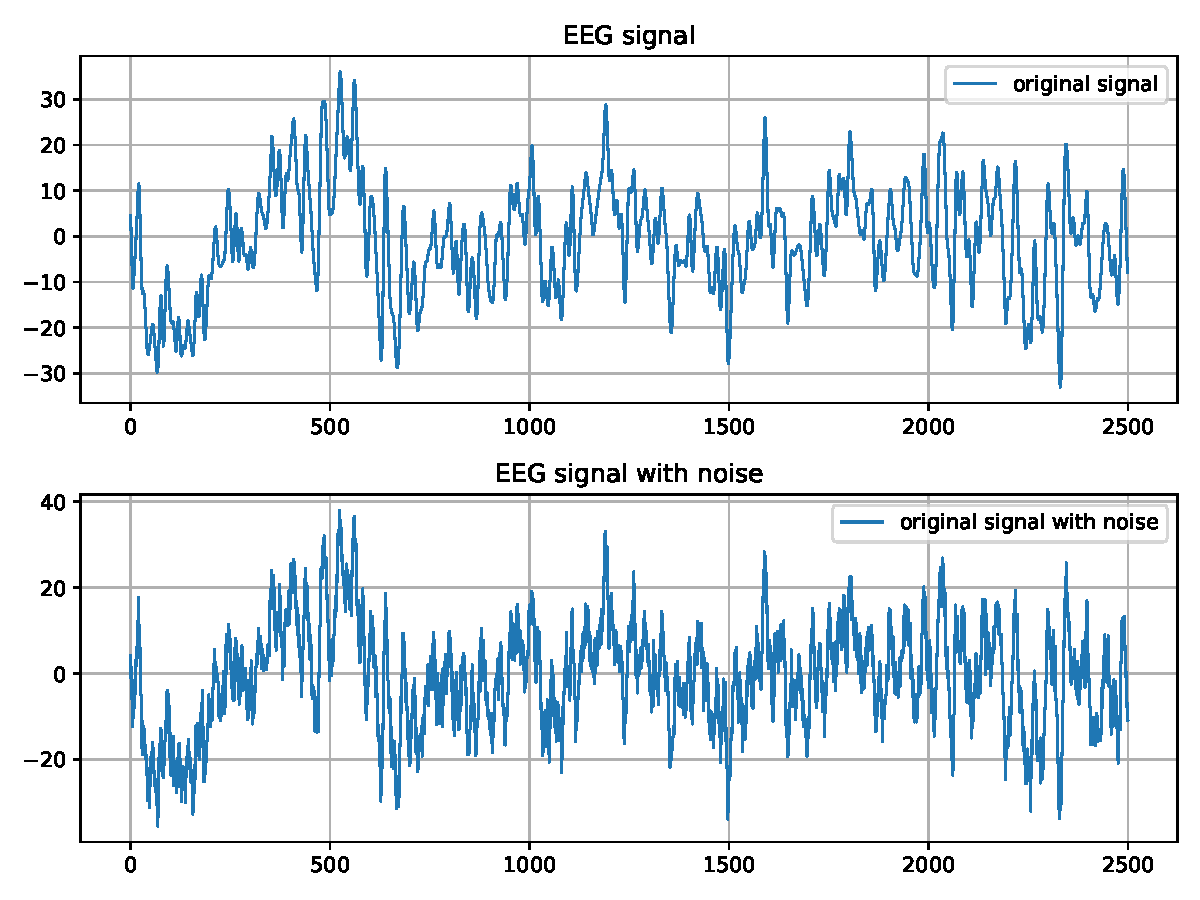
\includegraphics[width=\textwidth]{./img/problem2-1-EEG-signal-with-and-without-noise.pdf}
    \caption{The original EEG signal and its noisy version, where Gaussian noise with $\mu = 0$ and $\sigma = 3$ is added.}
    \label{fig:EEG_with_and_without_noise}
\end{figure}

\vspace{0.5cm}

\begin{tcolorbox}[colback=green!5!white,colframe=green!75!black,title=Problem 2.a]
    Compute signal to noise ratio (SNR).
\end{tcolorbox}

\begin{tcolorbox}[colback=green!5!white,colframe=green!75!black,title=Problem 2.b]
    Decompose the signal using wavedec (Haar, and db2).
\end{tcolorbox}

\begin{tcolorbox}[colback=green!5!white,colframe=green!75!black,title=Problem 2.c]
    Plot the subbands obtained using Haar and db2 decomposition.
\end{tcolorbox}

\begin{tcolorbox}[colback=green!5!white,colframe=green!75!black,title=Problem 2.d]
    Observe the subbands and list your observations.
\end{tcolorbox}


\ruler


\section*{Problem 3} \label{sec:problem3}

% problem introduction
\begin{tcolorbox}[colback=blue!5!white,boxrule=0pt,frame empty]
    Perform DWT on the given EEG signal (\verb|Q3.mat|) and threshold the detail coefficients
    the following way:
    \vspace{0.5em}
    \begin{itemize}
        \item Select a threshold $T = \sigma \sqrt{2 \log(n)}$ where n is the number of detail coefficients 
        and $\sigma$ is an estimate of the noise level.
        \item Set all detail coefficients smaller than $T$ to zero.
    \end{itemize}
\end{tcolorbox}


\vspace{0.5cm}

\begin{tcolorbox}[colback=blue!5!white,colframe=blue!75!black,title=Problem 3.a]
    Compute the SNR for different $\sigma$ values and values of $\sigma = \left \lbrace 0.5, 1, 2, 4 \right \rbrace$.
\end{tcolorbox}

\begin{tcolorbox}[colback=blue!5!white,colframe=blue!75!black,title=Problem 3.b]
    Plot the original, noisy, and denoised signal in anyone case.
\end{tcolorbox}


\begin{tcolorbox}[colback=blue!5!white,colframe=blue!75!black,title=Problem 3.c]
    Evaluate the RMSE and comment on your interpretations for each case.

\end{tcolorbox}
